\section{User Workflow}\label{chap:userWorkflow}


Nella seguente parte del documento verrà illustrato lo \textit{user flow} per le diverse tipologie di utenti del sistema WattGuard: utenti non autenticati, operatori tecnici e amministratori comunali. Le convenzioni grafiche utilizzate nel diagramma sono illustrate nella legenda in Figura \ref{fig:userWorkflowLegend}; 

\paragraph{Utenti non autenticati}
Come si può osservare in Figura \ref{fig:loginWorkflow}, gli utenti che non hanno ancora effettuato il login possono accedere alla pagina di autenticazione e alle pagine di recupero della password e di accettazione degli inviti; dalla pagina di autenticazione possono inoltre modificare la lingua dell'interfaccia (italiano, inglese o tedesco), con preferenza ricordata tra le sessioni. Dalla pagina di autenticazione l'utente può scegliere tra due modalità di accesso: l'inserimento di email e password con credenziali locali oppure l'autenticazione tramite Google, premendo il pulsante ``Accedi con Google''. Se le credenziali inserite sono valide, il sistema identifica il ruolo dell'utente (operatore tecnico o amministratore) e lo reindirizza alla dashboard generale dell'applicazione; in caso contrario vengono visualizzati messaggi di errore appropriati. Nel caso in cui l'utente abbia dimenticato la password, può richiederne il reset dall'apposita pagina e ricevere via email un link temporaneo (monouso, valido un'ora) per impostarne una nuova; se invece ha ricevuto un invito, può accettarlo tramite il link ricevuto, impostando la propria password al primo accesso oppure accettando con Google. Tutte le comunicazioni avvengono tramite protocollo HTTPS.


\paragraph{Operatori tecnici}
Dopo il login, l'operatore tecnico accede alla \textit{dashboard generale} come si può osservere in Figura \ref{fig:operatoreWorkflow}, che fornisce una panoramica aggregata dello stato del sistema: sensori attivi e totali, allarmi attivi e consumi correnti di elettricità e gas, con l'andamento temporale dei consumi; la dashboard si aggiorna automaticamente ogni 90 secondi (intervallo configurabile). Da qui l'operatore può cercare gli edifici utilizzando criteri multipli (nome, indirizzo, tipologia di edificio), ottenendo per ciascun risultato nome, indirizzo, tipologia impianto e stato operativo, e selezionare un edificio per visualizzarne il dettaglio completo: dati anagrafici, misurazioni in tempo reale (temperatura interna, esterna, consumo istantaneo), grafici storici con selezione di intervalli (giornaliero, settimanale, mensile, annuale, o tra due date distinte) e lo stato di funzionamento dei sensori. Il monitoraggio in tempo reale dei dati di ogni edificio avviene con aggiornamento automatico ogni 90 secondi, inclusi i grafici delle ultime 24 ore. L'operatore può inoltre consultare lo storico dei dati di un edificio selezionando l'attributo di interesse (temperatura, consumo, efficienza) e l'intervallo temporale, e visualizzare lo stato operativo di tutti i sensori installati, con evidenziazione dei sensori offline e la data dell'ultimo aggiornamento. Gestisce le notifiche di allarme tramite un pannello dedicato: visualizza tutti gli allarmi attivi ordinati per timestamp, consulta i dettagli di ciascun allarme e le soglie superate, li prende in carico e li chiude dopo la risoluzione. Configura inoltre le soglie di allarme dei sensori (valore minimo e massimo, ad esempio per temperatura e consumi): le soglie sono associate ai singoli sensori e possono quindi variare in base all'edificio e alla grandezza monitorata. Gestisce infine gli edifici: aggiungendo nuovi edifici con i relativi sensori (le coordinate geografiche vengono ricavate automaticamente dall'indirizzo tramite geocoding, con possibilità di modifica manuale), modificando le informazioni di quelli esistenti e rimuovendo gli edifici dismessi, con conferma e cancellazione a cascata di sensori, allarmi e rilevazioni associate. Le operazioni di creazione e modifica di edifici e sensori sono tracciate; per gli allarmi il sistema registra l'operatore e il timestamp di presa in carico e di risoluzione.


\paragraph{Amministratori comunali}
L'amministratore, dopo il login, accede alla stessa dashboard generale dell'operatore tecnico e dispone di tutte le funzionalità di quest'ultimo (gestione e monitoraggio di edifici, sensori, allarmi e soglie), ma con funzionalità aggiuntive per la gestione del sistema e l'analisi avanzata come si vede dalla Figura \ref{fig:amministratoreWorkflow}. Gestisce gli utenti e gli inviti: può creare nuovi inviti per operatori e amministratori specificando email e ruolo; il sistema invia all'utente un'email con il link di invito univoco e, al primo accesso, l'utente imposta la propria password oppure accetta l'invito tramite Google; l'amministratore può inoltre modificare il ruolo degli utenti esistenti, disabilitare o eliminare gli account e revocare gli inviti pendenti. Può esportare i dati dei consumi energetici in formato CSV selezionando uno o più edifici e il periodo temporale di interesse: il file generato contiene timestamp, edificio, sensore, tipologia, valore e unità di misura ed è formattato per l'importazione in fogli di calcolo; sono disponibili inoltre report aggregati in formato PDF ed Excel ed esportazioni in formato JSON (rilevazioni e backup del database). Tramite il pannello di configurazione del sistema, riservato all'amministratore, può esportare le rilevazioni in formato JSON, generare un backup completo del database e configurare i giorni di conservazione delle rilevazioni storiche (retention). Può infine confrontare le performance energetiche di più edifici (fino a tre), affiancando gli indicatori di efficienza termica calcolati dal sistema per ciascun edificio, in modo da identificare gli edifici più e meno efficienti e orientare le priorità di intervento.


\paragraph{Note sul flusso generale}
Le operazioni che richiedono delle autorizzazioni specifiche (ad esempio la gestione degli utenti o l'esportazione dei dati) sono protette a livello di ruolo. Il sistema garantisce l'accessibilità seguendo le linee guida WCAG 2.1 di livello A ed inoltre utilizza tecniche di caching intelligente per garantire tempi di caricamento rapidi (dashboard entro 10 secondi per il 95\% delle richieste); le performance sono mantenute anche con 20 utenti simultanei.

\begin{figure}[htbp]
    \centering
    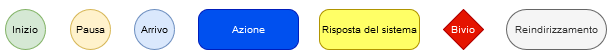
\includegraphics[width=0.9\textwidth]{../images/User_workflow/legendeUF.png}
    \caption{User Workflow Legend}
    \label{fig:userWorkflowLegend}
\end{figure}


\begin{figure}[htbp]
    \centering
    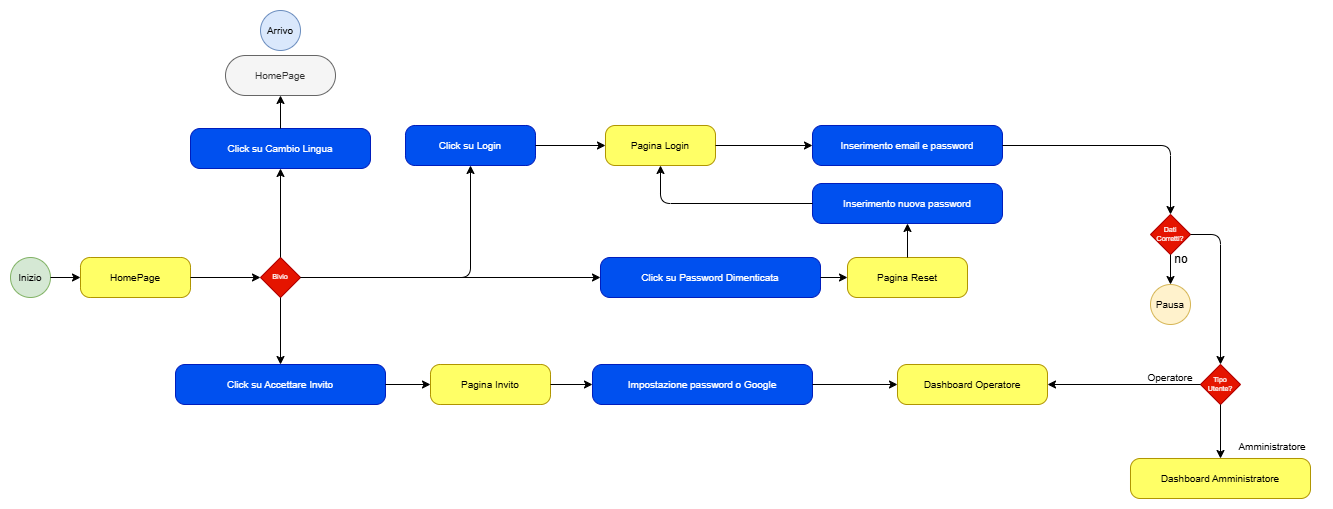
\includegraphics[width=\textwidth]{../images/User_workflow/UserFlowWattGuard-Login.drawio.png}
    \caption{Login Workflow - WattGuard}
    \label{fig:loginWorkflow}
\end{figure}

\begin{figure}[htbp]
    \centering
    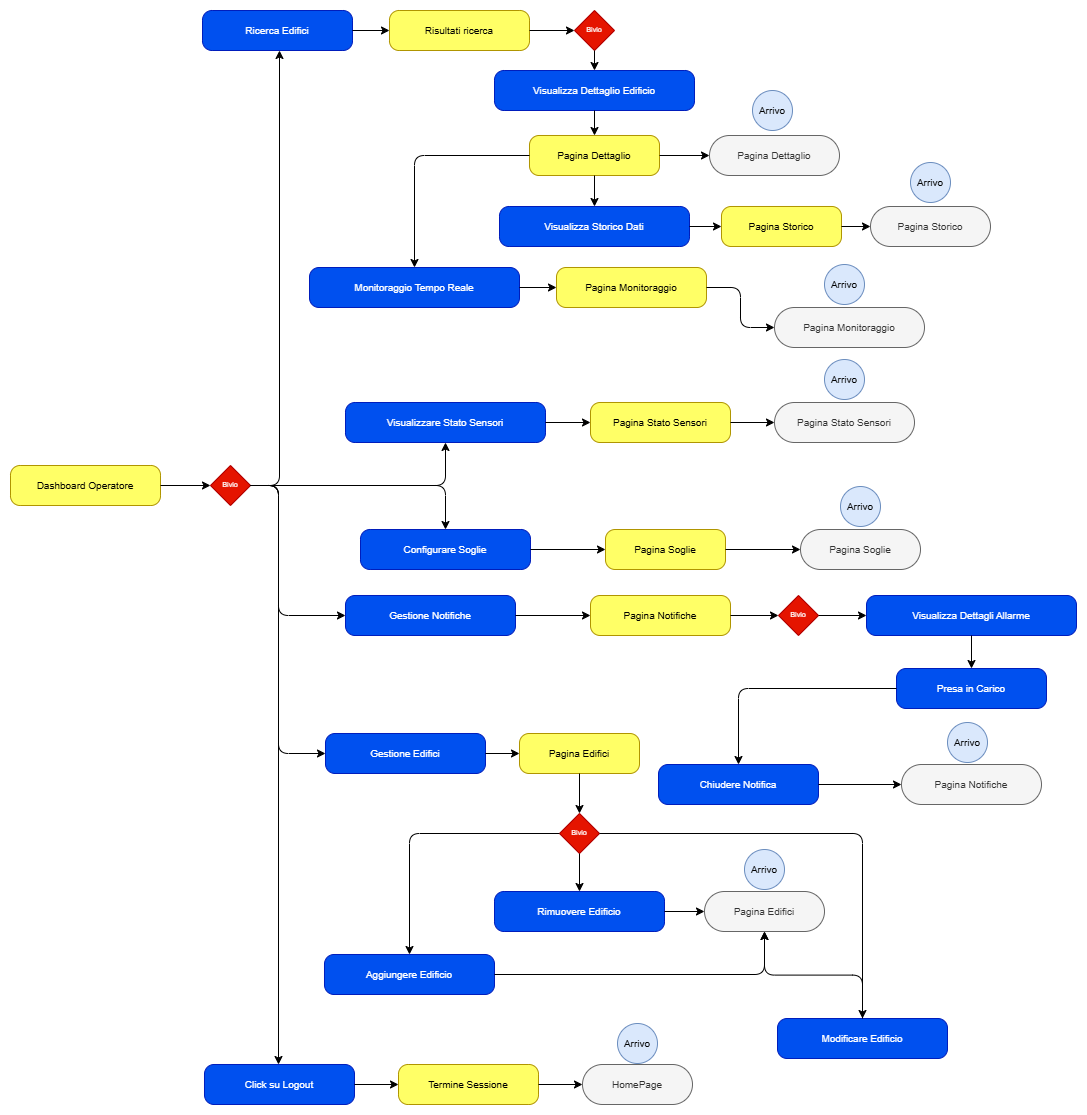
\includegraphics[width=\textwidth]{../images/User_workflow/UserFlowWattGuard-Operatore.drawio.png}
    \caption{Operatore Workflow - WattGuard}
    \label{fig:operatoreWorkflow}
\end{figure}

\begin{figure}[H]
    \centering
    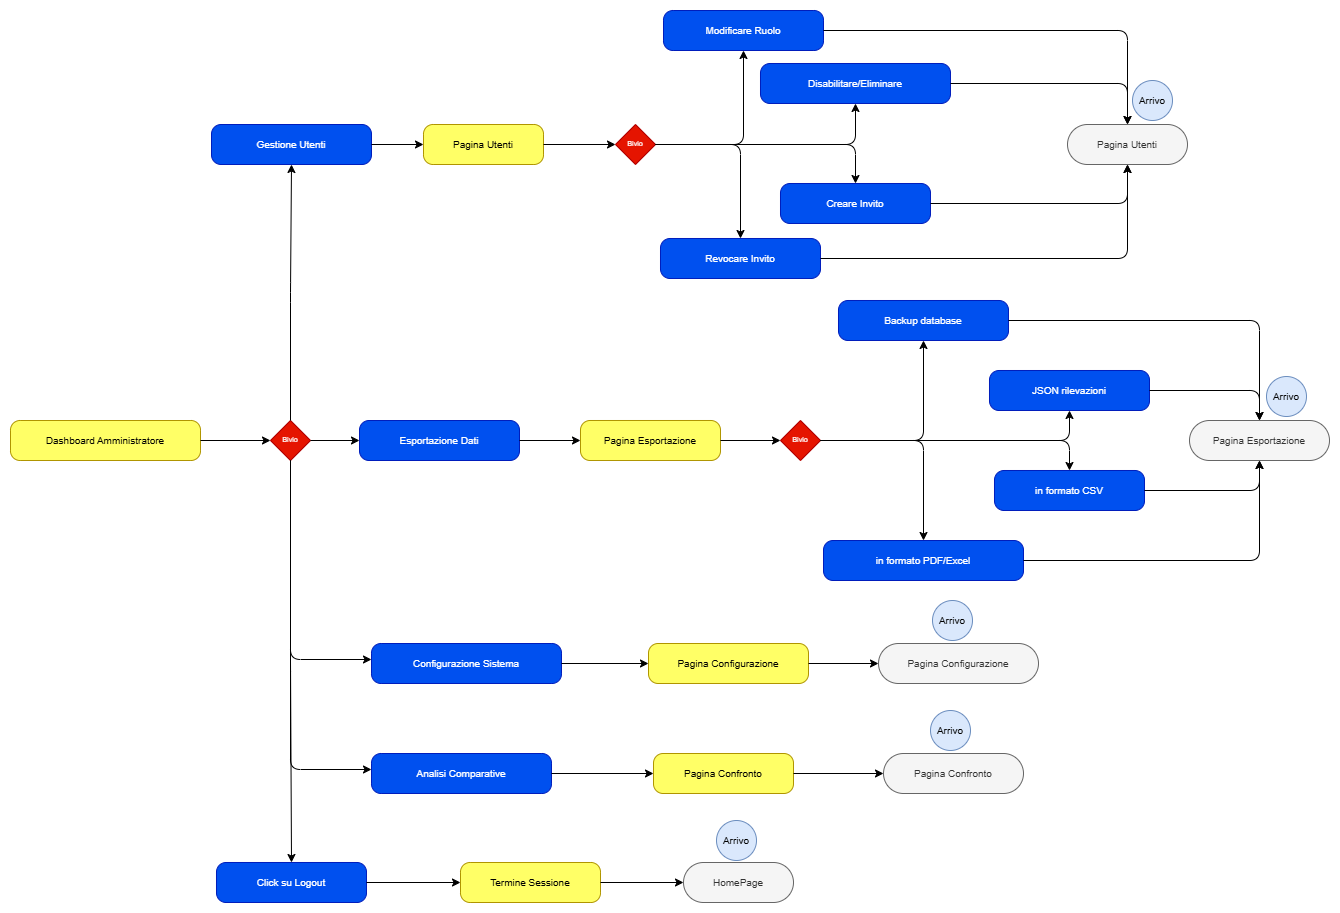
\includegraphics[width=\textwidth, height=0.5\textheight, keepaspectratio]{../images/User_workflow/UserFlowWattGuard-Amministratore.drawio.png}
    \caption{Amministratore Workflow - WattGuard}
    \label{fig:amministratoreWorkflow}
\end{figure}